\documentclass[11pt,a4paper]{article}
\usepackage[a4paper,margin=25mm,headheight=14pt,includeheadfoot]{geometry}
\usepackage[T1]{fontenc}
\usepackage[utf8]{inputenc}
\usepackage{lmodern}
\usepackage{microtype}
\usepackage{amsmath,amssymb,amsthm,mathtools}
\usepackage{booktabs,tabularx,longtable,array,multirow}
\usepackage{graphicx}
\usepackage{xcolor}
\usepackage{enumitem}
\usepackage{fancyhdr}
\usepackage{caption,subcaption}
\usepackage[numbers,sort&compress]{natbib}
\usepackage{hyperref}
\usepackage{float}
\usepackage{placeins}
\definecolor{ink}{HTML}{17324D}
\definecolor{teal}{HTML}{168C8C}
\definecolor{coral}{HTML}{C95C54}
\hypersetup{colorlinks=true,linkcolor=ink,citecolor=teal,urlcolor=teal,pdftitle={Decoding Deep Time Through a Diagenetic Channel},pdfauthor={Devanik Debnath}}
\pagestyle{fancy}\fancyhf{}\fancyhead[L]{\small\textcolor{ink}{DECODING DEEP TIME THROUGH A DIAGENETIC CHANNEL}}\fancyhead[R]{\small\thepage}\renewcommand{\headrulewidth}{0.35pt}
\captionsetup{font=small,labelfont=bf,justification=raggedright,singlelinecheck=false}
\setlength{\parskip}{0.35em}\setlength{\parindent}{1.1em}
\setlist{nosep,leftmargin=1.4em}
\newtheorem{proposition}{Proposition}
\newtheorem{definition}{Definition}
\title{\vspace{-1.2em}\textbf{Decoding Deep Time Through a Diagenetic Channel}\\[0.45em]
\large An Information-Theoretic Recoverability Framework for Speleothem Climate Archives}
\author{Devanik Debnath\\\small National Institute of Technology Agartala, India\\\small Research-process coordination: Xylia}
\date{18 October 2026\\[0.2em]\small Theoretical and computational preprint; not peer reviewed}
\begin{document}
\maketitle
\begin{abstract}
Speleothem records preserve valuable evidence about past hydroclimate, but measured isotope ratios, trace elements, biomarkers, and chronologies are mediated by karst transport, cave processes, biomediation, post-depositional alteration, and measurement error. Existing proxy-system models and petrographic workflows address important parts of this forward process, while Bayesian multi-proxy reconstructions quantify uncertainty from multiple records. This paper develops a complementary, falsifiable framework: treat the archive as a structured observation channel and ask whether climate is recoverable from the measured proxies when the channel state is only partially observed. The framework combines a linearized multi-proxy response model, a latent alteration state, and noisy fabric labels as side information. It derives an explicit identifiability condition, a Gaussian information-gain expression, and a fail-closed rule for reporting or withholding reconstructions. A reproducible synthetic benchmark compares single-proxy, multi-proxy, and fabric-informed linear decoders on held-out synthetic cave sequences under matched and shifted alteration. In this deliberately assumed simulator, channel-aware decoding modestly lowers RMSE relative to a multi-proxy baseline (0.2686 versus 0.2739 in-distribution; 0.3007 versus 0.3132 under the specified shift), but nominal 90\% prediction-interval coverage falls to 84.7\% under shift. The experiment therefore supports a methodological warning more strongly than a performance claim: side information can help, yet distribution shift and label noise can still produce undercoverage. No SISAL rows, SISAL\_monv1 monitoring records, or laboratory measurements were analyzed. A 2026 discussion preprint describes SISAL\_monv1, a potentially relevant global cave-monitoring compilation, but it is under review and its linked repository presented an anti-bot challenge during this cycle; co-registered proxy, fabric, chronology, and target coverage was therefore not verified. Empirical validation remains a separate, unmet gate. The contribution is a testable recoverability framework and reproducible stress test, not a claim of a validated paleoclimate decoder.
\end{abstract}
\noindent\textbf{Keywords:} speleothems; proxy-system models; diagenesis; calcite fabrics; information theory; inverse problems; Bayesian reconstruction; uncertainty calibration; paleoclimate

\section{Research posture and contribution}
A speleothem is not a tape recorder that maps climate variables directly to measured proxy values. Rainfall amount and isotope composition are filtered by soil and karst storage; dripwater chemistry and cave temperature influence precipitation; growth and fabric respond to hydrology, supersaturation, particles, organic compounds, and biological processes; and post-depositional change can alter geochemistry or chronology. This forward complexity is documented in proxy-system models, fabric logging, and studies of diagenesis \citep{CaveCalc2018,Frisia2015,Scholz2014,PSMAssessment2021}. A reconstruction is an inverse problem: from the remaining observations, infer the climate history and quantify the ambiguity.

We ask: \emph{under what conditions do multiple proxy records plus fabric-side information constrain climate more than the proxies alone, and when is the information loss too severe for a decoder to recover it?} The answer should not be “use a larger generative model by default.” A flexible decoder may regularize an ill-posed inverse problem, but it cannot manufacture identifying information absent from the observations. It may also be confidently wrong when the modern calibration domain and the deep-time archive differ.

\paragraph{Contribution.} This work proposes (i) a structured-channel observation model that separates climate response from alteration and measurement error; (ii) a response-geometry identifiability condition; (iii) information and uncertainty quantities conditional on fabric metadata; (iv) a reproducible synthetic stress test against transparent baselines; and (v) a preregisterable empirical protocol with explicit failure criteria. The framework formalizes and connects established ideas; it does not establish that a novel physical diagenetic process exists, nor that an AI decoder has recovered real paleoclimate.

\paragraph{Novelty posture.} Frisia's systematic microstratigraphic logging already turns fabrics into coded time series that can help distinguish hydrological, biomediation, and diagenetic influences \citep{Frisia2015}. CaveCalc and other proxy-system models already forward-model multiple chemical and isotope systems through cave processes \citep{CaveCalc2018}. Bayesian approaches already combine multiple paleoclimate archives and return probabilistic reconstructions \citep{Cahill2023}. Diagenetic alteration and U-series age effects have long been investigated, including models of uranium gain/loss and age inversions \citep{Scholz2014}. The limited claim here is the explicit synthesis of these pieces into a recoverability-first evaluation rule, paired with a synthetic comparison that tests both error and uncertainty under a declared channel shift. The literature search is not exhaustive; no absolute priority claim is made.

\section{Evidence base and closest prior work}
\subsection{What existing records and methods support}
SISALv3 is a major global compilation of speleothem stable isotope and trace-element records, reporting data from 365 sites and providing updated records and associated resources \citep{Kaushal2024SISALv3}. This scale is important for comparative reconstruction, but a geochemical compilation is not automatically a supervised machine-learning table: models require compatible observations of targets, proxy time series, chronologies, fabrics/alteration labels, and cave monitoring variables at appropriate temporal support. SISALv3's published description does not guarantee a unified, per-sample fabric label plus modern instrumental climate target for every record. A 2026 discussion preprint introduces SISAL\_monv1, a global cave-monitoring compilation with potentially relevant observations, including dripwater and cave monitoring \citep{Treble2026SISALMon}. The linked repository could not be inspected in this execution because it returned an anti-bot proof-of-work challenge; the paper and public abstract do not establish how many observations co-register with speleothem proxies and standardized fabric labels at matching temporal support. We therefore identify SISAL\_monv1 as a promising feasibility resource, not as an analyzed or confirmed training table. A field-by-field data audit is required before empirical work begins.

The Krem Mawmluh study of fatty acids reported evidence consistent with compounds arising from both cave microbial activity and overlying soil sources, and observed covariation with other biomarkers and isotope proxies; it also called for more analytical reference points \citep{Kalpana2021}. This demonstrates that biological material can carry environmental information and mixed provenance—not that every biomarker is noise or that microbial effects can be subtracted with a universal model. Similarly, diagenesis can affect uranium-series chronology and produce age inversions; its effects depend on alteration history and geochemical conditions \citep{Scholz2014}. These processes should be represented as candidate channel states with uncertain mappings, not collapsed into one undifferentiated error term.

\begin{table}[!htbp]\centering\small
\caption{Closest literature and the scope of the present framework. “What remains” identifies the narrower work proposed here, not an assertion that prior work is inadequate.}\label{tab:prior}
\begin{tabularx}{\linewidth}{p{0.22\linewidth}p{0.37\linewidth}X}\toprule
Research line & Established contribution & Remaining question addressed here \\\midrule
SISALv3 \citep{Kaushal2024SISALv3} & Global stable-isotope and trace-element compilation across 365 sites & Is the subset with aligned fabrics, chronology, monitoring, and proxy observations actually sufficient for supervised tests? \\
Fabric logging \citep{Frisia2015} & Microstratigraphic fabric coding as contextual evidence about growth, hydrology, biomediation, and diagenesis & When does an imperfect fabric label measurably improve climate identifiability? \\
Diagenesis and U-series dating \citep{Scholz2014} & Petrographic evidence and models linking alteration to age biases and inversions & How should alteration-state uncertainty propagate jointly into climate and age interpretation? \\
Forward proxy models \citep{CaveCalc2018,PSMAssessment2021} & Process-based mapping from hydrology/cave processes to chemistry and isotopes & What information about climate remains after the forward channel is inverted with side information? \\
Bayesian multi-proxy time series \citep{Cahill2023} & Probabilistic reconstructions combining natural archives & How should channel-state shift and explicit recoverability limits affect the permission to report a reconstruction? \\
Microbial biomarkers \citep{Kalpana2021} & Evidence for mixed soil/cave sources of fatty acids in a speleothem context & How can provenance labels be treated as uncertain evidence rather than a categorical “proxy valid/invalid” switch? \\
\bottomrule\end{tabularx}\end{table}

\subsection{Novelty and nearest-neighbour search}
Searches conducted on 18 October 2026 included title phrases and combinations of “speleothem,” “diagenesis,” “fabric,” “microbial,” “proxy-system model,” “Bayesian,” “information theory,” “inverse,” “generative,” and “machine learning,” plus the newly surfaced SISAL\_monv1 cave-monitoring preprint. These searches returned the closely related lines above but did not establish that no prior paper contains a channel-theoretic combination. Results are sensitive to indexing and terminology; therefore this is a documented scoped search, not a proof of priority. A specialist literature review and an empirical dataset audit are required before submission or stronger novelty language.

\section{Formal problem and epistemic status}
Let time index $t$ refer to latent climate variability at a selected temporal resolution, not directly to calendar time. Let $x_t\in\mathbb{R}^{d_x}$ denote the climate quantity or low-dimensional climate state of interest; $\mathbf y_t\in\mathbb{R}^{p}$ the measured geochemical/biomarker vector; $z_t$ a latent alteration state including diagenetic and microbial components; and $f_t$ observed fabric/texture metadata. Chronology is represented by a separate latent mapping $a(t)$ between sample depth/order and calendar age. The framework permits missing, irregularly sampled observations.

\begin{table}[!htbp]\centering\small
\caption{Core notation and units. The synthetic experiment standardizes variables; an empirical implementation must retain physical units and proxy-specific measurement models.}\label{tab:notation}
\begin{tabularx}{\linewidth}{p{0.17\linewidth}X p{0.31\linewidth}}\toprule
Symbol & Meaning & Status in this paper \\\midrule
$x_t$ & Latent climate target (e.g., standardized rainfall anomaly) & Synthetic truth in simulation; not measured paleoclimate \\
$\mathbf y_t$ & Vector of proxy observations & Three synthetic channels; not SISAL records \\
$z_t$ & Latent alteration/microbial channel state and magnitude & Simulated nuisance process \\
$f_t$ & Observed fabric label or petrographic side information & Noisy label of a 3-state synthetic class \\
$A$ & Climate-to-proxy response matrix & Assumed in toy forward model \\
$B$ & Alteration response subspace/loading matrix & Assumed in toy forward model \\
$\epsilon_t$ & Residual measurement/process error & Gaussian in the simplified model \\
$a(t)$ & Age-depth mapping or chronology posterior & Not estimated by the synthetic benchmark \\
$\Sigma_{x\mid y,f}$ & Conditional posterior covariance in Gaussian case & Analytical expression under stated assumptions \\
$I(x;\mathbf y\mid f)$ & Proxy information about climate conditional on fabric & Model-based diagnostic, not estimated from real data \\
\bottomrule\end{tabularx}\end{table}

\subsection{A structured observation channel}
A local linear approximation to a nonlinear proxy-system model is
\begin{equation}\label{eq:forward}
\mathbf y_t = A x_t + B_d z_{d,t} + B_m z_{m,t} + \boldsymbol\epsilon_t,
\end{equation}
where $z_{d,t}$ is a diagenetic state and $z_{m,t}$ a microbial/provenance state. With a vector climate target, $A x_t$ generalizes naturally to $A\mathbf x_t$. Coefficients can vary with cave, temperature, hydrology, mineralogy, or time; the constant-matrix form is a local approximation, not a universal physical law.

Fabric metadata provides side information through a noisy measurement model,
\begin{equation}\label{eq:fabric}
p(f_t\mid z_{d,t},z_{m,t},h_t),
\end{equation}
where $h_t$ contains observed petrographic/stratigraphic covariates. Equation~\ref{eq:fabric} must be calibrated from real paired samples; without paired labels, a model cannot infer the physical meaning of a fabric category from its name alone. Fabric can be climate-informative as well as alteration-informative. Thus it should not automatically be treated as an exclusion flag or as a pure nuisance proxy.

A generative decoder seeks the posterior
\begin{equation}\label{eq:posterior}
p(\mathbf x,\mathbf z_d,\mathbf z_m,\mathbf a\mid \mathbf y,\mathbf f,\mathcal D),
\end{equation}
where $\mathcal D$ represents calibration records and priors. A practical model may be hierarchical and non-Gaussian, but its posterior is only interpretable to the extent that its likelihood, calibration domain, label process, and chronology model are justified. A diffusion or transformer prior is not required at the first validation stage: a transparent baseline is preferable until there are enough correctly aligned paired observations to support richer models.

\subsection{Identifiability before decoder scale}
\begin{proposition}[A sufficient ambiguity condition in a linear channel]
Suppose $\mathbf y=A\mathbf x+B\mathbf z+\boldsymbol\epsilon$, with no side information on $\mathbf z$, and there are nonzero vectors $\Delta\mathbf x$ and $\Delta\mathbf z$ such that $A\Delta\mathbf x=-B\Delta\mathbf z$. Then the noiseless observation is unchanged when $(\mathbf x,\mathbf z)$ is replaced by $(\mathbf x+\Delta\mathbf x,\mathbf z+\Delta\mathbf z)$. Therefore the observation alone cannot uniquely identify both states over a domain containing those alternatives.
\end{proposition}
\noindent\emph{Proof sketch.} Substitution gives $A(\mathbf x+\Delta\mathbf x)+B(\mathbf z+\Delta\mathbf z)=A\mathbf x+B\mathbf z$. The observed vector is identical. A prior can select between the alternatives but does not create new observational evidence; conclusions then depend on the prior.\hfill$\square$

This is a P1 algebraic statement conditional on the linear model, not a claim that any specific real cave has this degeneracy. Near-overlap between the column spaces of climate and nuisance response matrices produces practical ill-conditioning even if exact non-identifiability is absent. Diagnostics should report singular values, condition numbers, and sensitivity to plausible nuisance priors. Additional independent proxies help only if their response directions contain new information rather than simply more measurements of the same confounded combination.

\begin{figure}[!htbp]\centering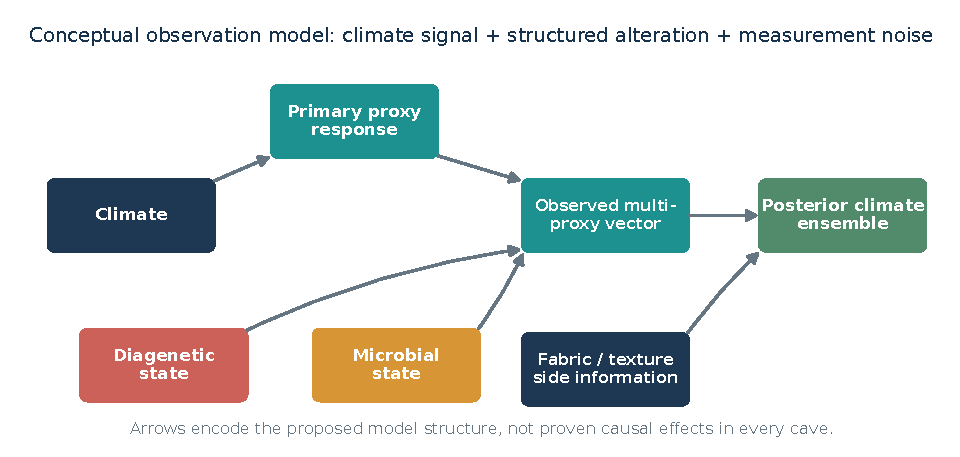
\includegraphics[width=0.94\linewidth]{figures/figure05_channel_dependency_graph.pdf}\caption{Proposed channel structure. Climate, diagenesis, microbial state, and fabric-side information jointly affect the inverse problem. The graph is a conceptual model diagram, not evidence that every arrow is causal or active in every cave.}\label{fig:channel}\end{figure}

\begin{figure}[!htbp]\centering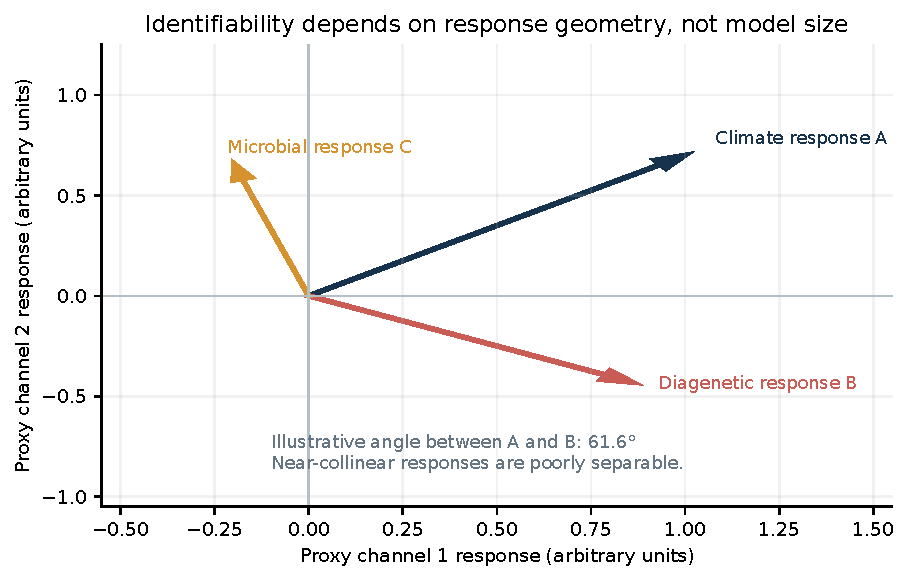
\includegraphics[width=0.72\linewidth]{figures/figure06_response_geometry_graph.pdf}\caption{Response geometry in a two-proxy projection using assumed loadings from the synthetic simulator. The angle is illustrative. Actual climate and alteration response directions would need to be estimated from paired observations, with uncertainty.}\label{fig:geometry}\end{figure}

\section{Information and uncertainty quantities}
For the transparent Gaussian case, suppose the prior on climate is $\mathbf x\sim\mathcal N(\boldsymbol\mu_x,\Sigma_x)$ and the conditional observation is $\mathbf y\mid\mathbf x,f\sim\mathcal N(A\mathbf x,\Sigma_n(f))$. Here $\Sigma_n(f)$ summarizes residual variation after conditioning on observed fabric and any fitted channel covariates. These formulas require a valid Gaussian model and known or estimated covariance matrices; an arbitrary fabric label does not automatically justify smaller noise variance.

The conditional covariance is
\begin{equation}\label{eq:cov}
\Sigma_{x\mid y,f}=\left(\Sigma_x^{-1}+A^\top\Sigma_n(f)^{-1}A\right)^{-1}.
\end{equation}
For a scalar climate target, covariance reduces to posterior variance. Comparing posterior variance with and without fabric-side information quantifies the contribution of the label, provided the two fits share the same validation data and account for the extra parameters.

Under the same Gaussian assumptions, the conditional mutual information is
\begin{equation}\label{eq:info}
I(\mathbf x;\mathbf y\mid f)=\frac12\log\det\!\left(I+\Sigma_x A^\top\Sigma_n(f)^{-1}A\right),
\end{equation}
measured in nats; divide by $\ln 2$ to express bits. This is the information that the proxy vector carries about the latent climate in the conditional Gaussian model. It is not a universal “climate information capacity,” and it is not directly estimable from SISAL metadata without a specified target distribution and calibrated likelihood.

A complementary rate--distortion view defines the minimum expected reconstruction distortion achievable at an information budget $R$:
\begin{equation}\label{eq:rd}
D^*(R)=\inf_{q(\hat{\mathbf x}\mid\mathbf y,\mathbf f):\ I(\mathbf y,\mathbf f;\hat{\mathbf x})\le R}
\mathbb E\left[d(\mathbf x,\hat{\mathbf x})\right].
\end{equation}
Here $d$ must be selected for the scientific task—for example squared error for standardized rainfall or an explicitly weighted loss for extremes and trend recovery. Rate--distortion is a conceptual performance frontier, not a claim that the present code estimates a physical channel capacity. The data-processing inequality further implies that a downstream decoder cannot recover information already discarded from its inputs; expressive neural architectures alter the estimator, not the evidence in the record.

\begin{table}[!htbp]\centering\small
\caption{Epistemological classification of the key claims. The P-level describes the type of support, not overall scientific importance.}\label{tab:epistemic}
\begin{tabularx}{\linewidth}{p{0.10\linewidth}p{0.30\linewidth}X}\toprule
Level & Claim class & Current status and boundary \\\midrule
P1 & Linear identifiability proposition; Gaussian posterior algebra & Exact conditional on explicit assumptions; says nothing by itself about physical validity \\
P2 & Bayesian regularization and optimal estimation & Model-dependent; estimator quality requires calibration and held-out tests \\
P3 & Stability of error/coverage under shifted channel states & Only tested in this synthetic simulator; no universal or empirical cave scaling inferred \\
P4 & Fabric as side information about channel state & Plausible formal correspondence grounded in fabric literature; label semantics and mapping are site-specific \\
P5 & “The archive is a noisy communication channel” metaphor & Useful framing only; physical interpretation depends on the forward model and observations \\
\bottomrule\end{tabularx}\end{table}

\section{Synthetic validation design}
\subsection{Purpose and simulator}
The first test is intentionally synthetic. It asks whether the proposed modeling distinctions behave as expected when the data-generating process is known, and exposes failure modes before real data are used. It does not establish that the synthetic loadings are representative of karst, calcite, microbes, or a climate regime.

Climate $x_t$ follows an autoregressive process with coefficient $\phi=0.78$. Three proxy channels use assumed climate loadings $(1.00,0.70,0.42)$, while alteration states add structured contributions with assumed diagenetic loadings $(0.86,-0.43,0.24)$ and microbial loadings $(-0.20,0.66,-0.78)$. Proxy-specific background noise has standard deviation 0.34. The three-state channel follows a persistent Markov-like sequence; fabric observations misclassify the true synthetic state at an assumed 10\% rate. Parameters are declared in \texttt{\detokenize{results/synthetic_generation_spec.json}}.

Training uses 72 synthetic caves by 170 time points (12,240 records). Two held-out scenarios each contain 20 synthetic caves by 170 time points (3,400 records): an in-distribution state mixture and a deliberately shifted alteration prevalence/scale. The split is by synthetic cave, not by randomly shuffled time points, to avoid an unrealistically easy within-cave leak. The current script fits ordinary least-squares estimators to: (1) one proxy; (2) all three proxies; (3) the same proxies plus one-hot observed fabric labels. Predictive intervals use a linear-model residual variance formula. They are reference intervals, not posterior intervals from a full hierarchical Bayesian model.

\begin{table}[!htbp]\centering\small
\caption{Synthetic experiment design. Every record and coefficient in this table is generated or assumed by the script; none is a measured cave datum.}\label{tab:design}
\begin{tabularx}{\linewidth}{p{0.30\linewidth}X}\toprule
Component & Specification \\\midrule
Random seed & 20261018 (fixed for the released run) \\
Training sample & 72 caves $\times$ 170 steps = 12,240 synthetic records \\
Held-out sample per scenario & 20 caves $\times$ 170 steps = 3,400 records \\
Climate process & Standardized AR(1), $\phi=0.78$ \\
Proxy channels & Three linear responses plus Gaussian background noise \\
Disturbance states & Nominal and altered prevalence with structured synthetic components \\
Observed fabric labels & 90\% assumed per-time-point classification accuracy \\
Comparators & Single-proxy OLS; three-proxy OLS; three-proxy plus fabric OLS \\
Primary metrics & RMSE, MAE, 90\% empirical coverage, mean interval width, Gaussian NLL \\
Empirical cave data & None imported; SISAL was not queried as a row-level dataset \\
\bottomrule\end{tabularx}\end{table}

\subsection{Prespecified acceptance gates}
A useful channel-aware decoder should improve held-out reconstruction error against the multi-proxy baseline by a practically stated margin, preserve or improve interval calibration, remain stable across held-out caves, and avoid spuriously narrow intervals under channel shift. For an empirical study, a proposed first gate is: cave-grouped held-out RMSE improvement of at least 5\% over the multi-proxy baseline, nominal 90\% interval coverage statistically compatible with 90\% on held-out caves, and no substantial worsening of log score. These thresholds are design choices and should be preregistered before viewing real held-out results. The current synthetic study is not expected to satisfy all gates by construction; failure is useful.

\begin{figure}[!htbp]\centering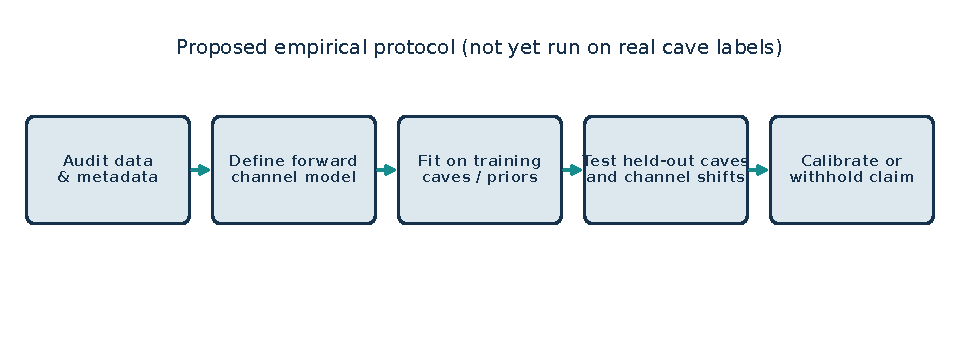
\includegraphics[width=0.92\linewidth]{figures/figure07_validation_pipeline_flow.pdf}\caption{Proposed real-data validation pipeline. The workflow is a proposal; no real-data fitting, held-out-cave analysis, or field test was performed in this release.}\label{fig:pipeline}\end{figure}

\section{Results of the synthetic stress test}
The main numerical outputs are recorded in \texttt{\detokenize{results/benchmark_metrics.csv}}. In-distribution, adding proxies substantially improves RMSE over the single-proxy model. Adding the noisy fabric label improves RMSE only modestly beyond the three-proxy baseline (0.2739 to 0.2686). In the shifted scenario, the channel-aware model also performs modestly better in RMSE than the multi-proxy baseline (0.3132 to 0.3007), but none of these values should be interpreted as performance on actual paleoclimate records.

\begin{table}[!htbp]\centering\small
\caption{Held-out synthetic performance. RMSE/MAE and uncertainty values are in standardized simulator units. $N=3{,}400$ per scenario. Coverage uses nominal 90\% Gaussian predictive intervals.}\label{tab:results}
\begin{tabular}{llrrrr}\toprule
Scenario & Method & RMSE & MAE & Coverage & NLL \\\midrule
In-distribution & Single proxy & 0.4289 & 0.3361 & 0.8853 & 0.5755 \\
In-distribution & Multi-proxy & 0.2739 & 0.2180 & 0.8956 & 0.1242 \\
In-distribution & Channel-aware & 0.2686 & 0.2135 & 0.8962 & 0.1047 \\
Shifted alteration & Single proxy & 0.6616 & 0.5346 & 0.6721 & 1.3442 \\
Shifted alteration & Multi-proxy & 0.3132 & 0.2510 & 0.8356 & 0.2813 \\
Shifted alteration & Channel-aware & 0.3007 & 0.2389 & 0.8471 & 0.2351 \\
\bottomrule\end{tabular}
\end{table}

\begin{figure}[!htbp]\centering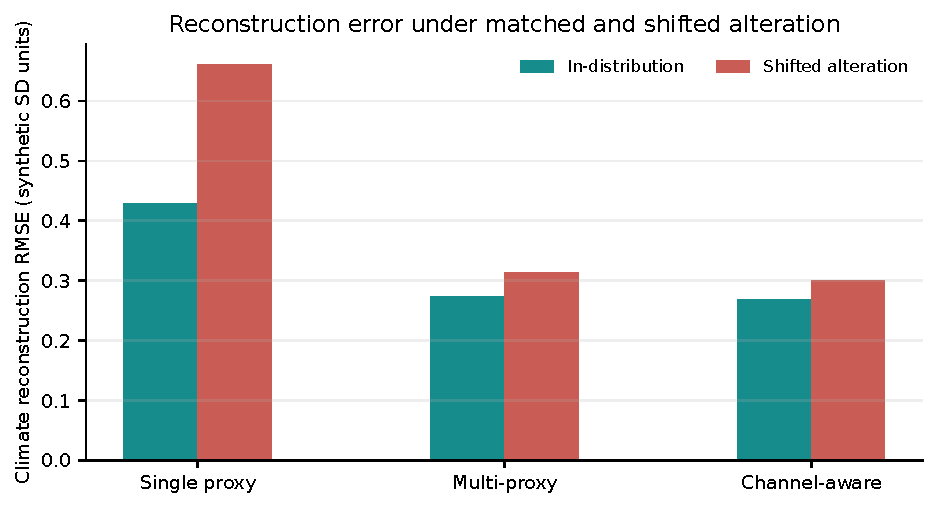
\includegraphics[width=0.90\linewidth]{figures/figure01_rmse_comparison.pdf}\caption{RMSE from the fixed-seed synthetic benchmark. Multi-proxy information dominates the single-proxy estimator; the additional gain from fabric labels is comparatively small. These are simulator outcomes only.}\label{fig:rmse}\end{figure}

\begin{figure}[!htbp]\centering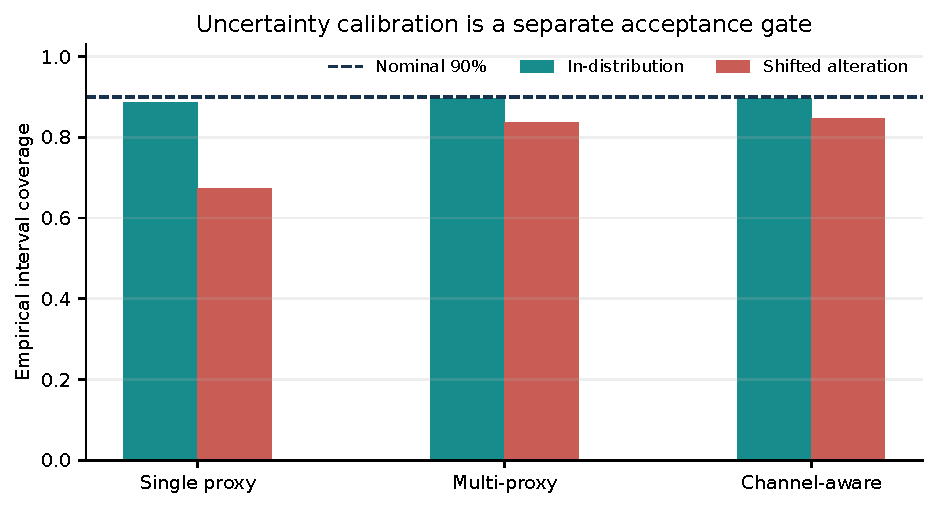
\includegraphics[width=0.90\linewidth]{figures/figure02_interval_coverage.pdf}\caption{Empirical coverage of nominal 90\% prediction intervals. Coverage drops under the shifted channel, demonstrating why improved point error cannot substitute for uncertainty validation.}\label{fig:coverage}\end{figure}

\begin{figure}[!htbp]\centering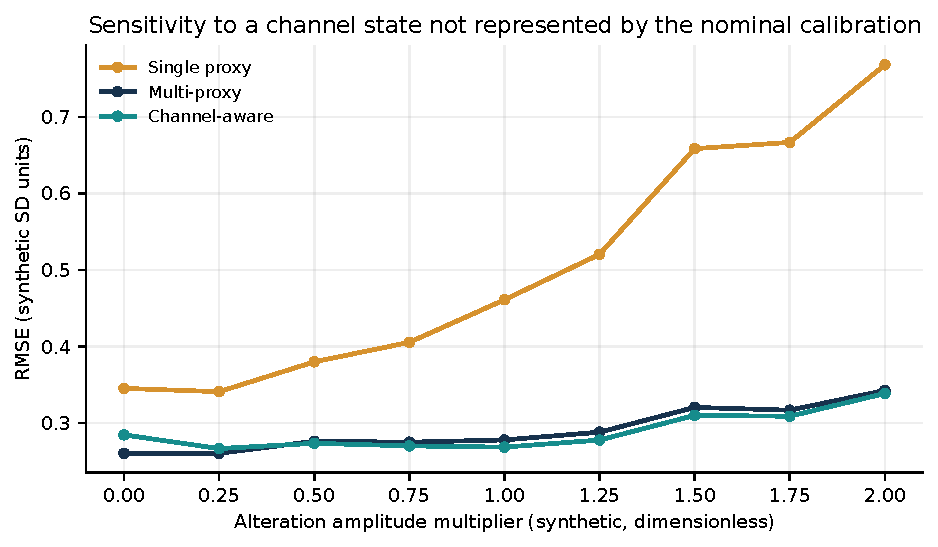
\includegraphics[width=0.90\linewidth]{figures/figure03_alteration_sensitivity.pdf}\caption{Sensitivity sweep in which the same estimators, fit under nominal conditions, are evaluated while the assumed alteration amplitude changes. The synthetic sweep is a stress test, not an estimate of alteration severity in nature.}\label{fig:sensitivity}\end{figure}

\begin{figure}[!htbp]\centering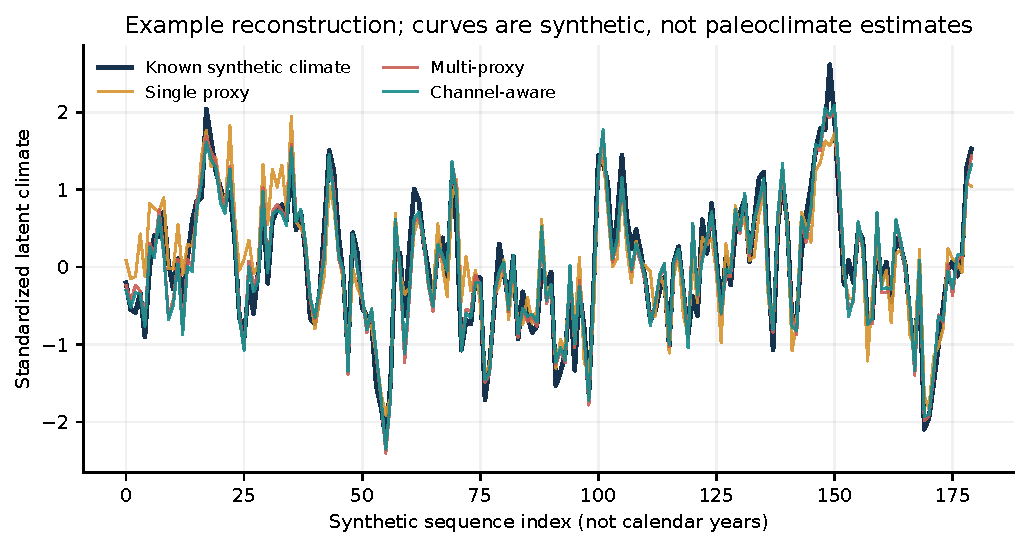
\includegraphics[width=0.93\linewidth]{figures/figure04_example_reconstruction.pdf}\caption{Single held-out synthetic time series. Curves compare the known latent process to the three estimates; the horizontal axis is a sequence index, not time in years. No real climate sequence is shown.}\label{fig:example}\end{figure}

\subsection{The calibration failure matters}
The channel-aware estimator has better point scores in both scenarios, but the shifted-scenario coverage is 84.7\%, below the nominal 90\%. The multi-proxy baseline reaches 83.6\%, and the single-proxy baseline collapses to 67.2\%. These gaps imply that a future real-data study must assess predictive intervals at the level of held-out caves and channel regimes. A model that “wins” by RMSE while delivering systematically overconfident intervals is not yet suitable for historical uncertainty statements.

\begin{table}[!htbp]\centering\small
\caption{Diagnostic interpretation of the synthetic outputs. These comparisons are descriptive; no across-cave confidence interval or inferential test is claimed.}\label{tab:diagnostics}
\begin{tabularx}{\linewidth}{p{0.28\linewidth}p{0.30\linewidth}X}\toprule
Finding & Computed evidence & Interpretation and limitation \\\midrule
Multiple proxies help & In-distribution RMSE: 0.4289 to 0.2739 from single to multi-proxy & Consistent with complementary simulated loadings; not evidence that any particular real proxy improves reconstruction \\
Fabric adds a small gain & In-distribution RMSE 0.2739 to 0.2686 & The model's label contains information by simulator construction; real label utility remains untested \\
Shift harms uncertainty & Channel-aware coverage 0.8962 to 0.8471 & The nominal model undercovers under distribution shift; interval width is not a guarantee \\
Single proxy is fragile & Shifted RMSE 0.6616 and coverage 0.6721 & This chosen simulator penalizes univariate decoding; do not generalize quantitatively \\
Error bars are model-based & Residual variance from fitted OLS & Does not include chronology, parameter, cave-level, or model-form uncertainty \\
\bottomrule\end{tabularx}\end{table}

\subsection{A worked-sequence view}
Figure~\ref{fig:example} plots one synthetic sequence to expose local behavior that aggregate metrics hide. It helps inspect whether the model tracks low-frequency variation or follows proxy noise, but a single series is not a validation sample. An empirical version should summarize all held-out caves and stratify error by fabric sequence, alteration indicator, proxy completeness, chronology uncertainty, and climate regime.

\section{Sensitivity, competing explanations, and failure modes}
A channel-aware improvement has several possible explanations: genuinely useful side information; leakage through correlated labels; model flexibility; fortuitous loading geometry; or an overly benign synthetic label process. The released code uses a cave-grouped split, but all train and test sets are generated from the same fixed simulator family. The shift changes state prevalence and disturbance amplitude while retaining the assumed response loadings. More severe forms of shift—changed coefficients, entirely new mineralogy, non-linear proxy saturation, missing-not-at-random measurements, altered age-depth relations, or unseen fabrics—are not tested in this experiment.

\begin{table}[!htbp]\centering\small
\caption{Sensitivity and failure conditions to evaluate before a real-data claim.}\label{tab:failure}
\begin{tabularx}{\linewidth}{p{0.25\linewidth}p{0.34\linewidth}X}\toprule
Perturbation & Why it matters & Required response \\\midrule
Fabric misclassification & Labels may be ambiguous, inconsistently logged, or time-varying & Estimate label confusion from replicated petrography; test worst plausible confusion matrices \\
Alteration prevalence/scale shift & Modern calibration may not span deep-time archive states & Held-out cave/geology splits; report coverage and abstain under unsupported regimes \\
Climate/nuisance collinearity & Proxies may respond similarly to climate and diagenesis & Report rank/singular values and posterior sensitivity; declare non-identifiability where appropriate \\
Proxy missingness & Samples may be missing because they are altered or hard to assay & Model the observation process; compare missingness assumptions \\
Chronology distortion & Alteration can perturb U-series ages and therefore event timing & Propagate age-depth ensembles jointly or separately with explicit uncertainty \\
Nonstationary biological contribution & Microbial and soil signals may vary with hydrology and ecosystem state & Use site-specific provenance calibration, not a universal “microbial noise” coefficient \\
Prior dominance & A strong generative prior can yield plausible yet unsupported curves & Compare with weak priors, prior predictive checks, and negative-control targets \\
\bottomrule\end{tabularx}\end{table}

One alternative explanation is that conventional proxy-system models may already capture the relevant physical effects when sufficiently well calibrated. The proposed method should therefore compare not only against a single-proxy transfer function but also against best available process-based models and conventional multi-proxy Bayesian reconstructions. A learned decoder must not be declared superior merely because it is evaluated against a weak baseline.

\section{Proposed empirical study and falsification plan}
\subsection{Data gate before model selection}
The minimum viable real-data dataset must align: (1) proxy observations and sample locations; (2) usable age-depth ensembles; (3) standardized fabric and petrographic alteration labels tied to those samples; (4) modern cave monitoring or an external target appropriate to the reconstruction task; and (5) cave-level splits so measurements from one cave cannot appear in both calibration and test partitions. Before model fitting, create a data availability matrix by record and field. If paired fabric/alteration labels and instrumental targets do not coexist at adequate scale, do not quietly impute them from unrelated sites and treat the result as supervised validation. Instead perform a transparent feasibility study, label-model analysis, and synthetic experiment, and postpone claims about empirical decoding.

A realistic path is a two-part design. First, use modern monitored caves with overlapping rainfall, dripwater, cave temperature, and speleothem proxy data to estimate forward response distributions and test whether fabrics carry incremental information about channel state. Second, evaluate the posterior decoder on held-out caves, then on longer archives using age-model ensembles. The target variable needs to be specific: instrumental rainfall anomaly, rainfall isotope composition, effective moisture, cave dripwater isotope, or another quantity are not interchangeable targets.

\begin{figure}[!htbp]\centering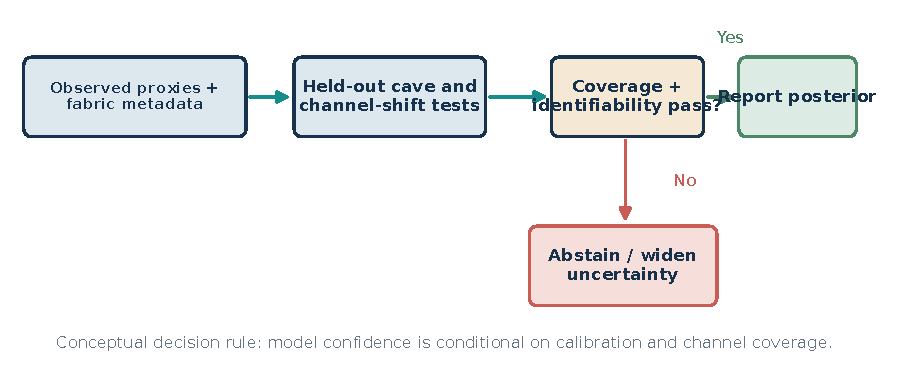
\includegraphics[width=0.89\linewidth]{figures/figure08_fail_closed_gate_flow.pdf}\caption{Fail-closed interpretation gate. If identifiability, calibration, or channel coverage is not established, the model must widen uncertainty or withhold a climate reconstruction rather than returning unjustifiably precise output.}\label{fig:gate}\end{figure}

\subsection{Predeclared pass and fail conditions}
A real-data study should register train/test cave assignments, comparator models, outcome metrics, missing-data handling, age uncertainty treatment, and threshold rules before opening test targets. The proposed primary metric is cave-grouped RMSE versus a strong multi-proxy baseline, accompanied by empirical coverage, mean interval width, continuous ranked probability score or log score, and calibration curves. Each cave is an independent grouping unit; thousands of within-cave time points must not be treated as thousands of independent caves.

\begin{table}[!htbp]\centering\small
\caption{Preregisterable empirical acceptance criteria. These are proposed design thresholds, not achieved results.}\label{tab:accept}
\begin{tabularx}{\linewidth}{p{0.27\linewidth}p{0.35\linewidth}X}\toprule
Gate & Proposed criterion & Fail action \\\midrule
Data provenance & Complete record-level source and field audit; no untracked labels & Restrict to the available-data claim and do not run supervised evaluation \\
Point accuracy & At least 5\% relative RMSE gain over strong multi-proxy baseline on held-out caves & Prefer simpler model; revise the channel structure \\
Uncertainty & 90\% interval coverage compatible with nominal coverage under cave-level resampling & Recalibrate, widen intervals, or abstain \\
Generalization & No unexplained large degradation by cave/geology/fabric subgroup & Report domain restriction and subgroup failure \\
Identifiability & Response geometry and posterior robust to reasonable prior changes & Mark climate component weakly identified or non-identifiable \\
Chronology & Climate inference stable across plausible age-depth ensembles & Separate timing claims from amplitude claims \\
Reproducibility & Frozen split, code, versions, manifest, and regenerated outputs match & Block release of empirical claim \\
\bottomrule\end{tabularx}\end{table}

The first falsification result would be a failure to improve predictive accuracy over a calibrated proxy baseline or a failure to maintain honest coverage on held-out caves. A second would be no incremental benefit from fabric metadata after accounting for the conventional forward model. A third would be extreme posterior sensitivity to priors under response collinearity. Any of these would justify reducing the method to a recoverability diagnostic rather than a generative climate decoder.

\section{Limitations and responsible interpretation}
The current code is a synthetic benchmark whose data-generating process is selected and known by construction. Its “climate,” “microbial,” “diagenetic,” and “fabric” variables have arbitrary standardized units and illustrative coefficients. It does not model isotope fractionation, karst residence-time distributions, calcite/aragonite transformation kinetics, real biomarker chemistry, U--Th isotopic equations, age-depth ensembles, speleothem growth, or actual cave monitoring. The three proxies are not calibrated proxies, the three-state fabric variable is not a petrographic taxonomy, and the reported prediction intervals omit major sources of uncertainty. Numerical success can only confirm that the implementation behaves consistently under this simulator.

The framework could be useful for better reconstruction of monsoon and regional hydroclimate variability if a calibrated forward model and reliable chronology support the inference. It could also identify archives where a quantitative climate signal cannot be separated from nuisance processes. But the path from this paper to any such benefit requires paired modern observations, lab-based mineralogical/geochemical analyses, independent chronology, careful model comparison, and community scrutiny. No direct human health, climate-policy, or engineering utility is claimed.

Ethical and epistemic safeguards include preserving original measurements, labeling inferred and observed values separately, documenting provenance and missingness, making uncertainty visible, and not replacing expert petrographic assessment with a black-box score. Model outputs should complement rather than overrule cave-specific geological interpretation.

\section{Conclusion}
Viewing speleothem reconstruction as a structured inverse channel is useful only if the model can identify what the archive actually preserves. This paper formalizes climate–alteration ambiguity, expresses the potential contribution of fabric-side information in a Gaussian baseline, and provides reproducible synthetic comparisons against single- and multi-proxy estimators. The modest synthetic accuracy gain and shifted-coverage failure indicate that adding a channel label does not eliminate uncertainty or guarantee calibration. The next decisive step is not a larger generative neural network; it is a data audit and held-out-cave validation with co-located fabrics, altered mineralogy indicators, chronology ensembles, and modern target measurements. Until those data are aligned and the empirical gates pass, the proposed method remains a falsifiable research framework rather than a validated paleoclimate reconstruction system.

\vspace{0.6em}\noindent\textbf{Research-process credit and responsibility.} Co-equal research-process credit is given to Devanik Debnath and Xylia, the autonomous multi-model research engine coordinating AI-assisted discovery, synthesis, and verification. Devanik Debnath retains responsibility for the final manuscript, scientific claims, citations, and released artifacts.

\section*{Reproducibility and data availability}
The repository release contains \texttt{\detokenize{verify_model.py}}, the fixed-seed synthetic generation specification, metrics CSV files, and the vector figure assets. Run \texttt{\detokenize{python verify_model.py}} with Python 3.10+, NumPy 1.24+, and Matplotlib 3.7+ to regenerate the synthetic benchmark and figures. No empirical dataset was downloaded or analyzed. SISALv3 and SISAL\_monv1 are identified as potential resources, but row-level co-registration and licensing/attribution requirements remain to be audited against their original sources before any real-data fit.

\bibliographystyle{plainnat}
\bibliography{paper}
\end{document}
